\documentclass{beamer}
\usetheme[
    numbering=none,
    progressbar=head,
]{metropolis}
\usepackage{graphicx}
\graphicspath{ {../report/img/} }

\title{On Parameterized Vertex Cover in Streaming}
\date{\today}
\author{Adam Cox}
\institute{
    School of Computer Science \\
    University of Birmingham
}

\begin{document}

\maketitle

\section{Quick crash course in Graph Theory}

\begin{frame}{Graph Theory}
    \begin{columns}
        \begin{column}{0.55\textwidth}
            \begin{block}{Nodes/Vertices}
                Representing objects
            \end{block}
            \begin{block}{Edges}
                Representing relationships between objects
            \end{block}
        \end{column}
        \begin{column}{0.35\textwidth}
            \begin{center}
                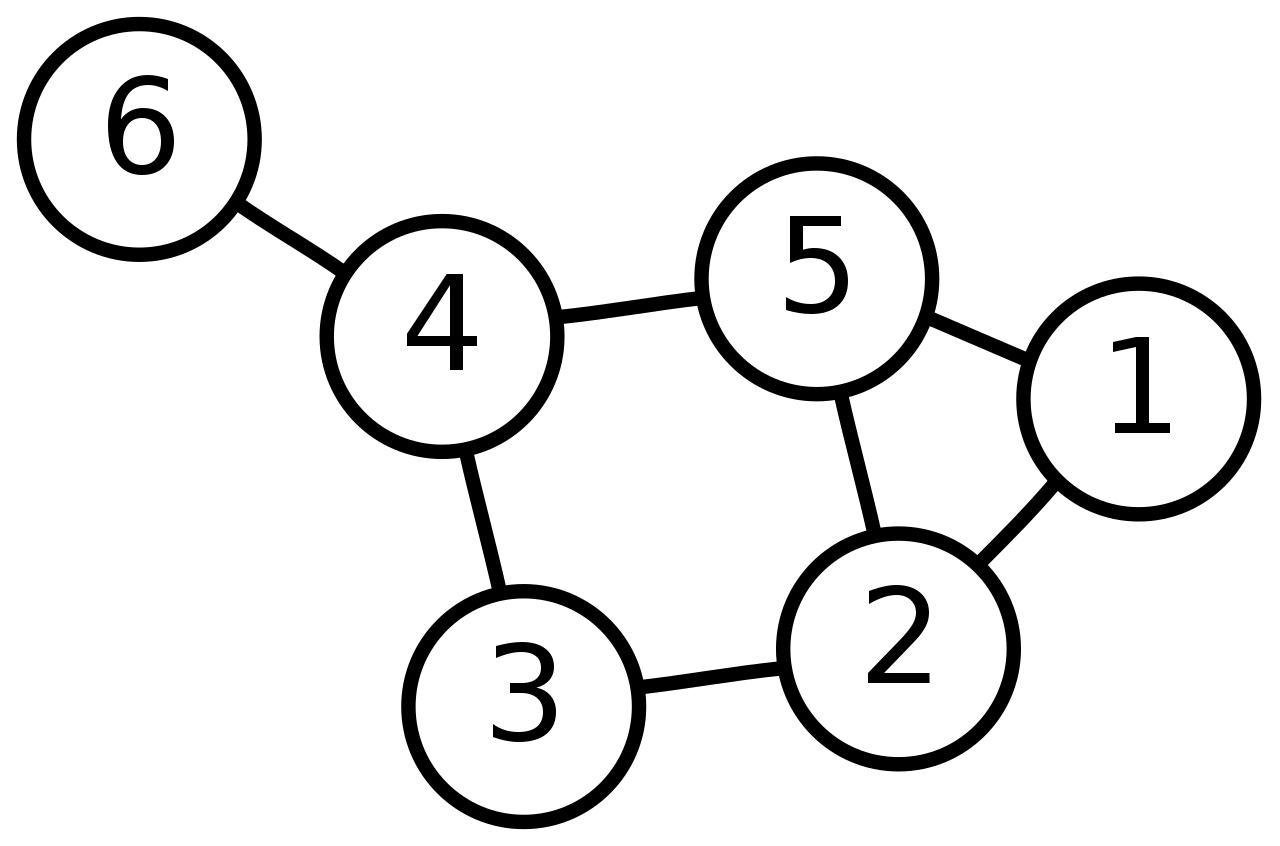
\includegraphics[width=\textwidth]{graph-theory}
            \end{center}
        \end{column}
    \end{columns}

    \begin{center}
        Together this makes a \textbf{graph}
    \end{center}
\end{frame}

\section{Let me break down the title}

\begin{frame}{On Parameterized \alert{Vertex Cover} in Streaming}
    \begin{columns}
        \begin{column}{0.6\textwidth}
            A set of vertices that includes at least one endpoint of every edge of the graph.

            \hfill

            Typically we want to find the \textbf{minimum} vertex cover.
        \end{column}
        \begin{column}{0.3\textwidth}
            \begin{center}
                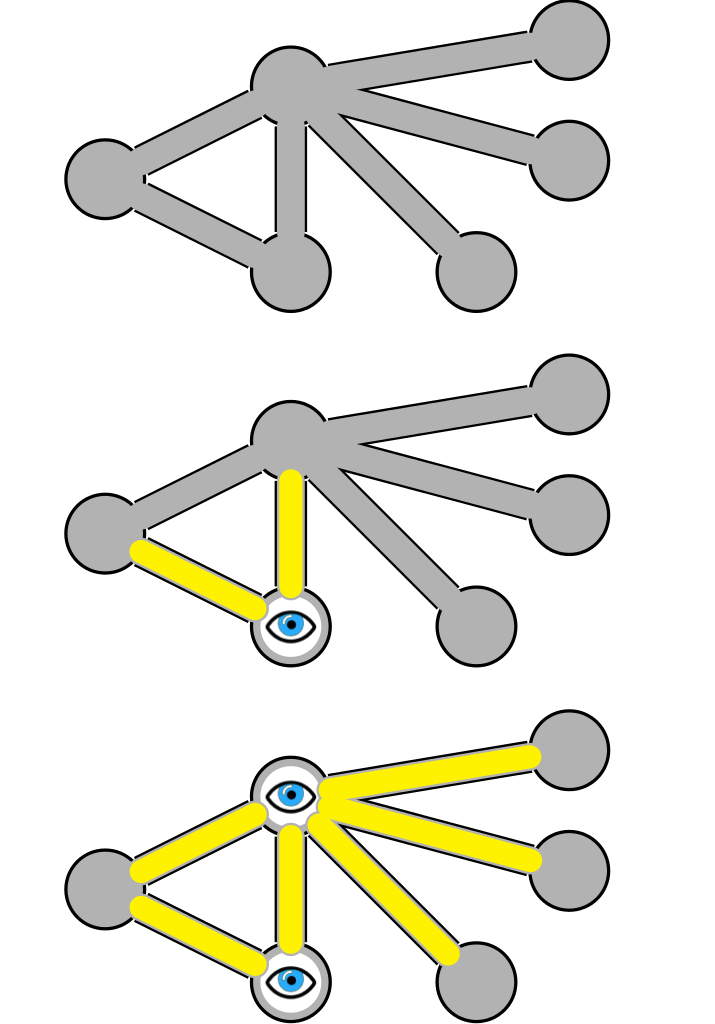
\includegraphics[width=\textwidth]{vertex-cover}
            \end{center}
        \end{column}
    \end{columns}
\end{frame}

\begin{frame}{On \alert{Parameterized} Vertex Cover in Streaming}
    Classical complexity measures runtime of an algorithm solely based on the input size

    Parameterized complexity allows for multiple parameters of the input or output

    Non-parameterized/classical TIME : 1960s

    parameterized TIME : 1990s
\end{frame}

\begin{frame}{On \alert{Parameterized Vertex Cover} in Streaming}
    This is known as the \textbf{Vertex Cover Problem} or k-VC

    \hfill

    \begin{alertblock}{k-VC}
        INSTANCE: Graph $G$ and positive integer $k$\\
        QUESTION: Does $G$ have a vertex cover of size at most $k$?\\
    \end{alertblock}

    \hfill

    The vertex cover problem is an NP-complete problem
\end{frame}

\begin{frame}{On Parameterized Vertex Cover in \alert{Streaming}}
    Big Data means it's too big to store/look at in one go. Therefore we need streaming.

    \hfill

    Non-parameterized SPACE :2000s

    parameterized SPACE :2015
\end{frame}

\begin{frame}{On \alert{Parameterized Vertex Cover in Streaming}}
    So for the full problem, we are looking at:

    \begin{itemize}
        \item insertion-only stream of edges
        \item value $k$
    \end{itemize}

    And we want a True/False answer.
\end{frame}

\section{Motivation}

\begin{frame}{Karp's 21 NP-complete problems}
    The vertex cover problem is an NP-complete problem: it was one of Karp's 21 NP-complete problems. It is often used in computational complexity theory as a starting point for NP-hardness proofs.
\end{frame}

\begin{frame}{If you need a physical example}
    Imagine a city with a highly complex road network. The city wants to set up cameras at junctions to be able to monitor every road. How would you calculate the most efficient placement of the cameras?

    \begin{itemize}
        \item Budget of cameras/money
    \end{itemize}
\end{frame}

\section{The Algorithms}

\begin{frame}{Historically}
    Branching and kernelization
\end{frame}

\begin{frame}{State of the Art}
    Rajesh Chitnis et al
\end{frame}

\section{My work}

\begin{frame}{Implementation}

\end{frame}

\begin{frame}{Testing}

\end{frame}

\begin{frame}{Visualisation}

\end{frame}

\begin{frame}[standout]
    Thank you
\end{frame}

\end{document}